%!TEX root = Thesis_main.tex

\addcontentsline{toc}{chapter}{Appendices}
\label{AppB}
\begin{figure}[!th]
	\begin{center} 
		\centerline{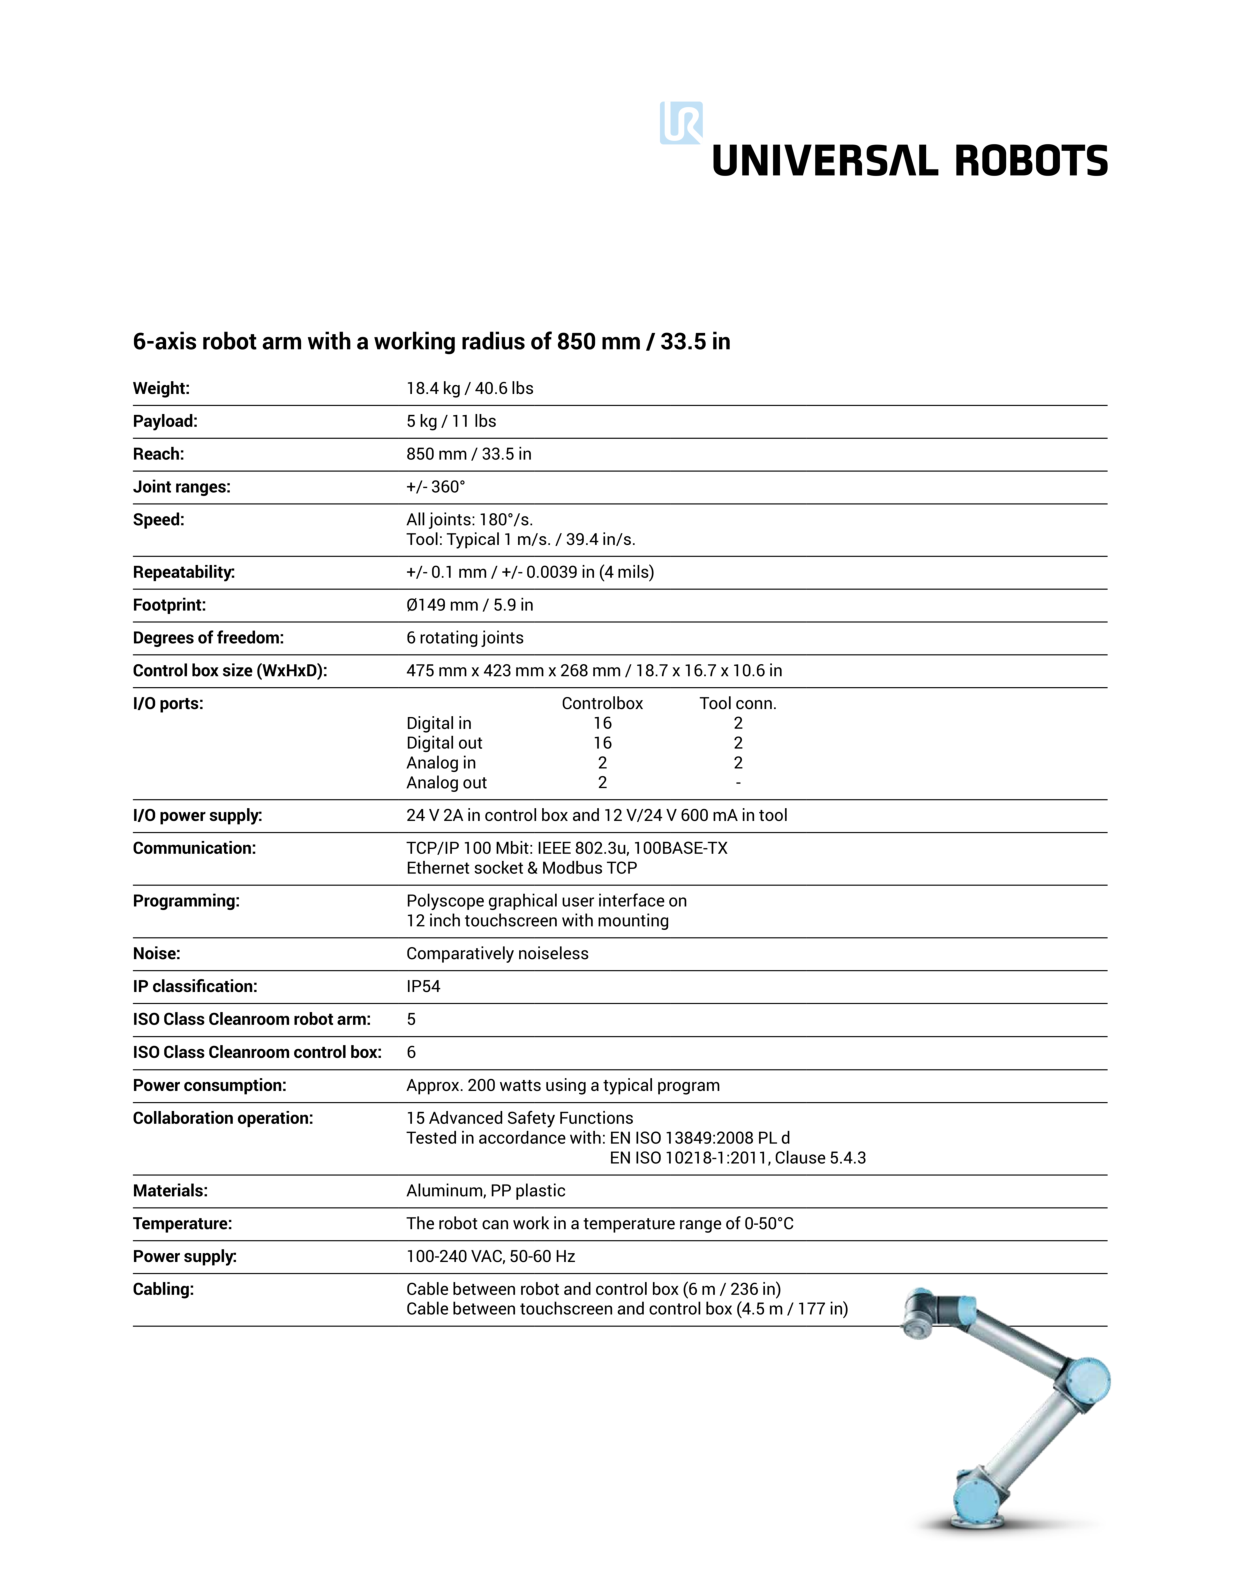
\includegraphics[scale=0.9]{ur5_en_V2}}
		\label{SMB Wiring} 
	\end{center}
\end{figure}


% In the following table the specifications given by Universal Robots are stated. 
% \begin{table}
% 	\begin{tabular}{p{4cm} | p{3cm} p{3cm}}
% 		\hline
% 		Performance & \multicolumn{2}{l}{ } \\
% 		\hline \hline
% 		Repeatibility & \multicolumn{2}{l}{$\pm$ 0.1 mm} \\
% 		Ambient temperature range & \multicolumn{2}{l}{0-50°} \\
% 		Power Consumption  & \multicolumn{2}{l}{Min 90W, Typical 150W, Max 325W} \\
% 		Collaboration operation & \multicolumn{2}{l}{15 advanced adjustable safety functions} \\
% 		\hline \hline
% 		Specifications & \multicolumn{2}{l}{ }\\
% 		\hline \hline 
% 		Payload & \multicolumn{2}{l}{5 kg} \\
% 		Reach & \multicolumn{2}{l}{850 mm} \\
% 		Degrees of freedom & \multicolumn{2}{l}{6 rotating joints} \\
% 		Programming & \multicolumn{2}{l}{Polyscope graphical user interface on 12 inch touchscreen} \\
% 		\hline \hline
% 		Movement & & \\
% 		\hline 
% 		& Working range & Maximum speed \\
% 		\hline \hline
% 		Base & $\pm$ 360°  & $\pm$ 180°/sec \\
% 		Shoulder & $\pm$ 360° & $\pm$ 180°/sec \\
% 		Wrist1 & $\pm$ 360° & $\pm$ 180°/sec \\
% 		Wrist2 & $\pm$ 360° & $\pm$ 180°/sec \\
% 		Wrist3 & $\pm$ 360° & $\pm$ 180°/sec \\
% 		Typical tool & & 1m/sec \\
% 		\hline \hline
% 		Physical & \multicolumn{2}{l}{ }\\
% 		\hline \hline
% 		Footprint & \multicolumn{2}{l}{\o 149mm} \\
% 		Materials & \multicolumn{2}{l}{Aluminium, PP Plastics} \\
% 		Weight (with cable) & 18.4 kg 
% 	\end{tabular}
% \end{table}